\uuid{w5fr}
\exo7id{7059}
\titre{exo7 7059}
\auteur{megy}
\organisation{exo7}
\datecreate{2017-01-11}
\isIndication{true}
\isCorrection{true}
\chapitre{Géométrie affine dans le plan et dans l'espace}
\sousChapitre{Propriétés des triangles}
\module{Géométrie}
\niveau{L2}
\difficulte{}

\contenu{
\texte{
% collège
% triangle rectangle, cercle circonscrit
Soit $ABC$ un triangle et $\mathcal C$ son cercle circonscrit, de centre $O$.
Soit $A’$ le point diamétralement opposé à $A$ sur le cercle $\mathcal C$.
La hauteur $(AH)$ issue de $A$ du triangle $ABC$ recoupe le cercle $\mathcal C$ au point $D$.

Montrer que la droite $(DA’)$ est parallèle à $(BC)$.
}
\indication{Le triangle rectangle $ADA’$ est inscrit dans un demi-cercle. 
% donc il y a un autre angle droit}
\reponse{
~\\
%\begin{center}
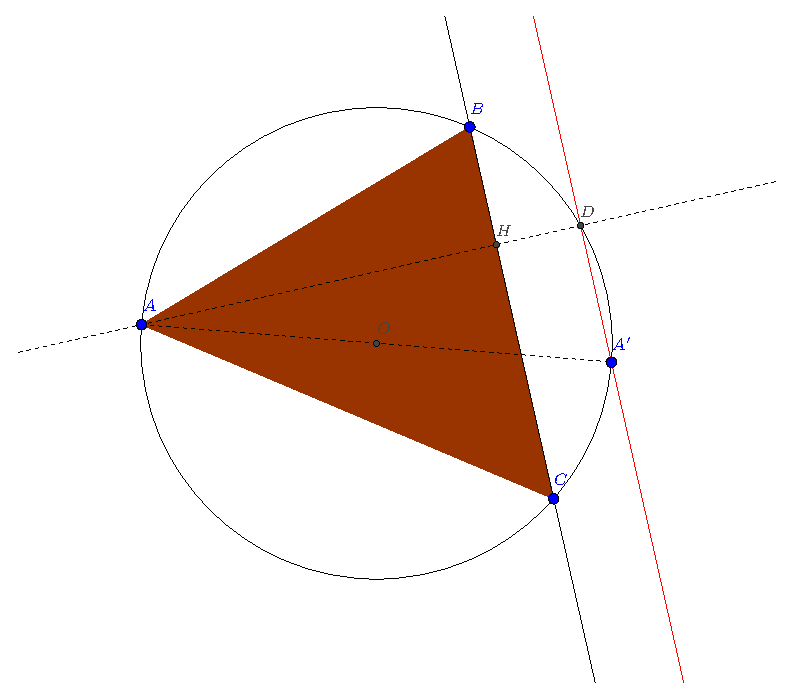
\includegraphics{../images/w5fr-1}
%\end{center}

D'après les hypothèses, la droite $(BC)$ est perpendiculaire à la droite $(AH)$ et $ADA'$ est rectangle en $D$. Donc, les droites $(AH)$ et $(A'D)$ sont perpendiculaires. Or, deux droites perpendiculaires à une même droite sont parallèles.
}
}
